% Options for packages loaded elsewhere
\PassOptionsToPackage{unicode}{hyperref}
\PassOptionsToPackage{hyphens}{url}
\PassOptionsToPackage{dvipsnames,svgnames,x11names}{xcolor}
%
\documentclass[
  letterpaper,
  DIV=11,
  numbers=noendperiod,
  oneside]{scrartcl}

\usepackage{amsmath,amssymb}
\usepackage{lmodern}
\usepackage{iftex}
\ifPDFTeX
  \usepackage[T1]{fontenc}
  \usepackage[utf8]{inputenc}
  \usepackage{textcomp} % provide euro and other symbols
\else % if luatex or xetex
  \usepackage{unicode-math}
  \defaultfontfeatures{Scale=MatchLowercase}
  \defaultfontfeatures[\rmfamily]{Ligatures=TeX,Scale=1}
\fi
% Use upquote if available, for straight quotes in verbatim environments
\IfFileExists{upquote.sty}{\usepackage{upquote}}{}
\IfFileExists{microtype.sty}{% use microtype if available
  \usepackage[]{microtype}
  \UseMicrotypeSet[protrusion]{basicmath} % disable protrusion for tt fonts
}{}
\makeatletter
\@ifundefined{KOMAClassName}{% if non-KOMA class
  \IfFileExists{parskip.sty}{%
    \usepackage{parskip}
  }{% else
    \setlength{\parindent}{0pt}
    \setlength{\parskip}{6pt plus 2pt minus 1pt}}
}{% if KOMA class
  \KOMAoptions{parskip=half}}
\makeatother
\usepackage{xcolor}
\usepackage[top=30mm,left=30mm]{geometry}
\setlength{\emergencystretch}{3em} % prevent overfull lines
\setcounter{secnumdepth}{-\maxdimen} % remove section numbering
% Make \paragraph and \subparagraph free-standing
\ifx\paragraph\undefined\else
  \let\oldparagraph\paragraph
  \renewcommand{\paragraph}[1]{\oldparagraph{#1}\mbox{}}
\fi
\ifx\subparagraph\undefined\else
  \let\oldsubparagraph\subparagraph
  \renewcommand{\subparagraph}[1]{\oldsubparagraph{#1}\mbox{}}
\fi

\usepackage{color}
\usepackage{fancyvrb}
\newcommand{\VerbBar}{|}
\newcommand{\VERB}{\Verb[commandchars=\\\{\}]}
\DefineVerbatimEnvironment{Highlighting}{Verbatim}{commandchars=\\\{\}}
% Add ',fontsize=\small' for more characters per line
\usepackage{framed}
\definecolor{shadecolor}{RGB}{241,243,245}
\newenvironment{Shaded}{\begin{snugshade}}{\end{snugshade}}
\newcommand{\AlertTok}[1]{\textcolor[rgb]{0.68,0.00,0.00}{#1}}
\newcommand{\AnnotationTok}[1]{\textcolor[rgb]{0.37,0.37,0.37}{#1}}
\newcommand{\AttributeTok}[1]{\textcolor[rgb]{0.40,0.45,0.13}{#1}}
\newcommand{\BaseNTok}[1]{\textcolor[rgb]{0.68,0.00,0.00}{#1}}
\newcommand{\BuiltInTok}[1]{\textcolor[rgb]{0.00,0.23,0.31}{#1}}
\newcommand{\CharTok}[1]{\textcolor[rgb]{0.13,0.47,0.30}{#1}}
\newcommand{\CommentTok}[1]{\textcolor[rgb]{0.37,0.37,0.37}{#1}}
\newcommand{\CommentVarTok}[1]{\textcolor[rgb]{0.37,0.37,0.37}{\textit{#1}}}
\newcommand{\ConstantTok}[1]{\textcolor[rgb]{0.56,0.35,0.01}{#1}}
\newcommand{\ControlFlowTok}[1]{\textcolor[rgb]{0.00,0.23,0.31}{#1}}
\newcommand{\DataTypeTok}[1]{\textcolor[rgb]{0.68,0.00,0.00}{#1}}
\newcommand{\DecValTok}[1]{\textcolor[rgb]{0.68,0.00,0.00}{#1}}
\newcommand{\DocumentationTok}[1]{\textcolor[rgb]{0.37,0.37,0.37}{\textit{#1}}}
\newcommand{\ErrorTok}[1]{\textcolor[rgb]{0.68,0.00,0.00}{#1}}
\newcommand{\ExtensionTok}[1]{\textcolor[rgb]{0.00,0.23,0.31}{#1}}
\newcommand{\FloatTok}[1]{\textcolor[rgb]{0.68,0.00,0.00}{#1}}
\newcommand{\FunctionTok}[1]{\textcolor[rgb]{0.28,0.35,0.67}{#1}}
\newcommand{\ImportTok}[1]{\textcolor[rgb]{0.00,0.46,0.62}{#1}}
\newcommand{\InformationTok}[1]{\textcolor[rgb]{0.37,0.37,0.37}{#1}}
\newcommand{\KeywordTok}[1]{\textcolor[rgb]{0.00,0.23,0.31}{#1}}
\newcommand{\NormalTok}[1]{\textcolor[rgb]{0.00,0.23,0.31}{#1}}
\newcommand{\OperatorTok}[1]{\textcolor[rgb]{0.37,0.37,0.37}{#1}}
\newcommand{\OtherTok}[1]{\textcolor[rgb]{0.00,0.23,0.31}{#1}}
\newcommand{\PreprocessorTok}[1]{\textcolor[rgb]{0.68,0.00,0.00}{#1}}
\newcommand{\RegionMarkerTok}[1]{\textcolor[rgb]{0.00,0.23,0.31}{#1}}
\newcommand{\SpecialCharTok}[1]{\textcolor[rgb]{0.37,0.37,0.37}{#1}}
\newcommand{\SpecialStringTok}[1]{\textcolor[rgb]{0.13,0.47,0.30}{#1}}
\newcommand{\StringTok}[1]{\textcolor[rgb]{0.13,0.47,0.30}{#1}}
\newcommand{\VariableTok}[1]{\textcolor[rgb]{0.07,0.07,0.07}{#1}}
\newcommand{\VerbatimStringTok}[1]{\textcolor[rgb]{0.13,0.47,0.30}{#1}}
\newcommand{\WarningTok}[1]{\textcolor[rgb]{0.37,0.37,0.37}{\textit{#1}}}

\providecommand{\tightlist}{%
  \setlength{\itemsep}{0pt}\setlength{\parskip}{0pt}}\usepackage{longtable,booktabs,array}
\usepackage{calc} % for calculating minipage widths
% Correct order of tables after \paragraph or \subparagraph
\usepackage{etoolbox}
\makeatletter
\patchcmd\longtable{\par}{\if@noskipsec\mbox{}\fi\par}{}{}
\makeatother
% Allow footnotes in longtable head/foot
\IfFileExists{footnotehyper.sty}{\usepackage{footnotehyper}}{\usepackage{footnote}}
\makesavenoteenv{longtable}
\usepackage{graphicx}
\makeatletter
\def\maxwidth{\ifdim\Gin@nat@width>\linewidth\linewidth\else\Gin@nat@width\fi}
\def\maxheight{\ifdim\Gin@nat@height>\textheight\textheight\else\Gin@nat@height\fi}
\makeatother
% Scale images if necessary, so that they will not overflow the page
% margins by default, and it is still possible to overwrite the defaults
% using explicit options in \includegraphics[width, height, ...]{}
\setkeys{Gin}{width=\maxwidth,height=\maxheight,keepaspectratio}
% Set default figure placement to htbp
\makeatletter
\def\fps@figure{htbp}
\makeatother

\KOMAoption{captions}{tableheading}
\makeatletter
\makeatother
\makeatletter
\makeatother
\makeatletter
\@ifpackageloaded{caption}{}{\usepackage{caption}}
\AtBeginDocument{%
\ifdefined\contentsname
  \renewcommand*\contentsname{Table of contents}
\else
  \newcommand\contentsname{Table of contents}
\fi
\ifdefined\listfigurename
  \renewcommand*\listfigurename{List of Figures}
\else
  \newcommand\listfigurename{List of Figures}
\fi
\ifdefined\listtablename
  \renewcommand*\listtablename{List of Tables}
\else
  \newcommand\listtablename{List of Tables}
\fi
\ifdefined\figurename
  \renewcommand*\figurename{Figure}
\else
  \newcommand\figurename{Figure}
\fi
\ifdefined\tablename
  \renewcommand*\tablename{Table}
\else
  \newcommand\tablename{Table}
\fi
}
\@ifpackageloaded{float}{}{\usepackage{float}}
\floatstyle{ruled}
\@ifundefined{c@chapter}{\newfloat{codelisting}{h}{lop}}{\newfloat{codelisting}{h}{lop}[chapter]}
\floatname{codelisting}{Listing}
\newcommand*\listoflistings{\listof{codelisting}{List of Listings}}
\makeatother
\makeatletter
\@ifpackageloaded{caption}{}{\usepackage{caption}}
\@ifpackageloaded{subcaption}{}{\usepackage{subcaption}}
\makeatother
\makeatletter
\@ifpackageloaded{tcolorbox}{}{\usepackage[many]{tcolorbox}}
\makeatother
\makeatletter
\@ifundefined{shadecolor}{\definecolor{shadecolor}{rgb}{.97, .97, .97}}
\makeatother
\makeatletter
\@ifpackageloaded{sidenotes}{}{\usepackage{sidenotes}}
\@ifpackageloaded{marginnote}{}{\usepackage{marginnote}}
\makeatother
\makeatletter
\makeatother
\ifLuaTeX
  \usepackage{selnolig}  % disable illegal ligatures
\fi
\IfFileExists{bookmark.sty}{\usepackage{bookmark}}{\usepackage{hyperref}}
\IfFileExists{xurl.sty}{\usepackage{xurl}}{} % add URL line breaks if available
\urlstyle{same} % disable monospaced font for URLs
\hypersetup{
  pdftitle={Introduction to Deep Neural Networks},
  colorlinks=true,
  linkcolor={blue},
  filecolor={Maroon},
  citecolor={Blue},
  urlcolor={Blue},
  pdfcreator={LaTeX via pandoc}}

\title{Introduction to Deep Neural Networks}
\author{}
\date{5/3/23}

\begin{document}
\maketitle
\ifdefined\Shaded\renewenvironment{Shaded}{\begin{tcolorbox}[borderline west={3pt}{0pt}{shadecolor}, sharp corners, boxrule=0pt, enhanced, breakable, frame hidden, interior hidden]}{\end{tcolorbox}}\fi

\renewcommand*\contentsname{Table of contents}
{
\hypersetup{linkcolor=}
\setcounter{tocdepth}{3}
\tableofcontents
}
\begin{Shaded}
\begin{Highlighting}[]
\FunctionTok{options}\NormalTok{(}\AttributeTok{width=}\DecValTok{100}\NormalTok{) }
\ControlFlowTok{if}\NormalTok{(}\SpecialCharTok{!}\FunctionTok{require}\NormalTok{(}\StringTok{"knitr"}\NormalTok{)) }\FunctionTok{install.packages}\NormalTok{(}\StringTok{"knitr"}\NormalTok{)}
\FunctionTok{library}\NormalTok{(}\StringTok{"knitr"}\NormalTok{)}
\CommentTok{\#getOption("width")}
\NormalTok{knitr}\SpecialCharTok{::}\NormalTok{opts\_chunk}\SpecialCharTok{$}\FunctionTok{set}\NormalTok{(}\AttributeTok{comment=}\ConstantTok{NA}\NormalTok{,}\AttributeTok{echo =} \ConstantTok{TRUE}\NormalTok{, }\AttributeTok{cache=}\ConstantTok{TRUE}\NormalTok{)}
\end{Highlighting}
\end{Shaded}

\hypertarget{introduction-to-deep-neural-networks}{%
\section{Introduction to Deep Neural
Networks}\label{introduction-to-deep-neural-networks}}

\hypertarget{overview-of-deep-learning}{%
\subsection{Overview of Deep Learning}\label{overview-of-deep-learning}}

\hypertarget{historical-background-and-key-milestones}{%
\subsubsection{Historical Background and Key
Milestones}\label{historical-background-and-key-milestones}}

Today, in April 2023, our world is convulsed by the explosion of
Artificial Intelligence.

Although it has been growing steadily, it has probably been in the last
months (weeks), since ChatGPT has arrived, that everybody has an
opinion, or a fear on the topic.

\begin{figure}

{\centering \includegraphics{https://bernardmarr.com/wp-content/uploads/2022/04/The-Dangers-Of-Not-Aligning-Artificial-Intelligence-With-Human-Values.jpg}

}

\end{figure}

While we are not going to discuss ethical, technological or sociological
aspects, what seems clear to the data scientist's eye is that
``\emph{most of this is about prediction}''.

Most AI engines rely on powerful prediction systems that use statistical
learning methods.

Deep learning is a highly successful model in the field of AI, which has
powered numerous applications in various domains. It has shown
remarkable performance in tasks such as image recognition, natural
language processing, and speech recognition.

Deep learning extends the basic principles of artificial neural networks
by introducing more complex architectures and algorithms and, at the
same time, by enabling machines to learn from large datasets by
automatically identifying relevant patterns and features without
explicit programming.

One key advantage of deep learning over traditional machine learning
algorithms is its ability to handle high-dimensional and unstructured
data such as images, videos, and audio.

\hypertarget{the-early-history-of-artificial-neural-networksintelligence}{%
\subsubsection{The early history of artificial {[}neural
networks{]}/intelligence}\label{the-early-history-of-artificial-neural-networksintelligence}}

\begin{figure}

{\centering 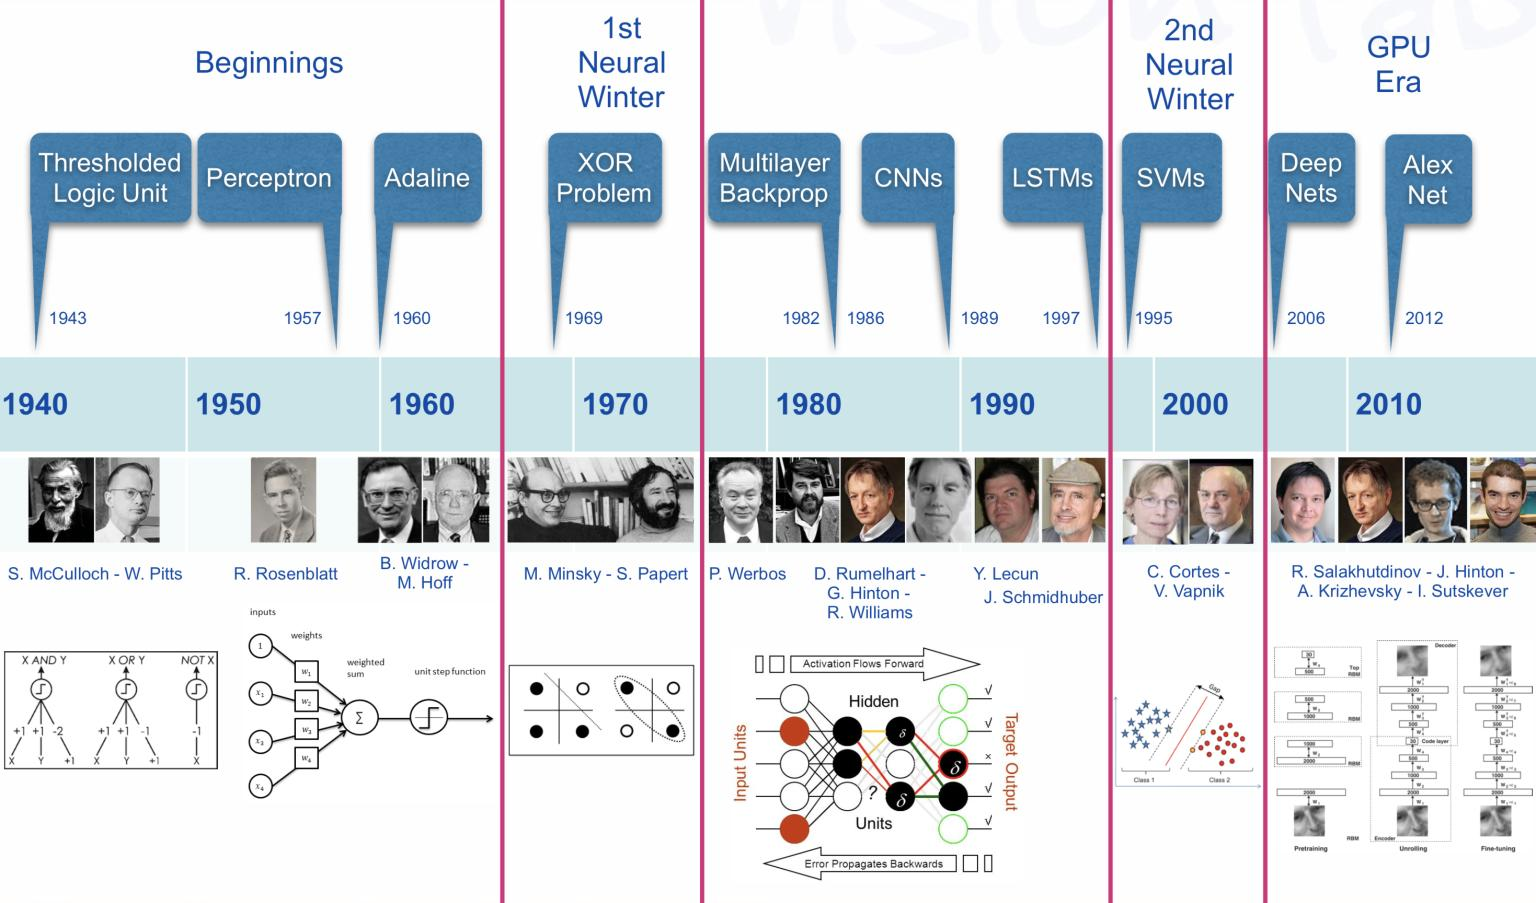
\includegraphics{images/AIHistory1.jpg}

}

\caption{A Brief History of AI from 1940s till Today}

\end{figure}

\begin{figure}

{\centering 

\href{https://nerdyelectronics.com/a-quick-history-of-ai-ml-and-dl/}{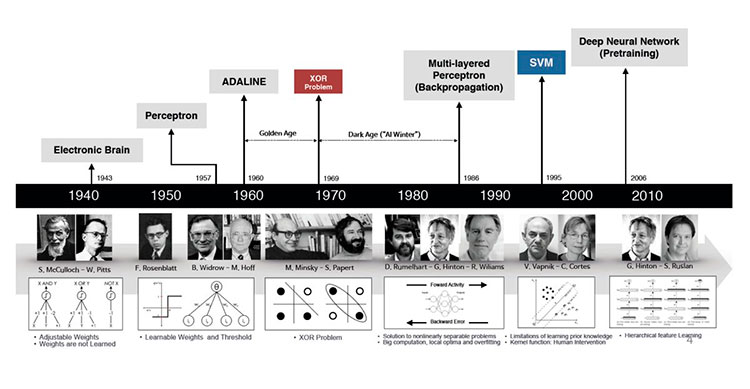
\includegraphics{images/AIHistory2.jpg}}

}

\caption{The origins of Deep learning and modern Artificial Intelligence
can be traced back to the per4ceptron. Source: ``A Quick History of AI,
ML and DL''}

\end{figure}

The origins of AI, and as such of DL can be traced almost one century
backwards. While it is an interesting, or even fascinating, history wee
don't go into it (see a summary in
\protect\hypertarget{AIHistory}{\href{https://nerdyelectronics.com/a-quick-history-of-ai-ml-and-dl/}{A
Quick History of AI, ML and DL}}

We can see there however, several hints worth to account for because we
will go through them to understand how a deep neural network works.
These are:

\begin{itemize}
\item
  The \textbf{Perceptron} and the first \textbf{Artificial Neural
  Network} where the basic building block was introduced.
\item
  The \textbf{Multilayered perceptron} and \textbf{backpropagation}
  where complex architechtures were suggested to improve the
  capabilities.
\item
  \textbf{Deep Neural Networks}, with many hidden layers, and
  auto-tunability capabilities.
\end{itemize}

In short, there has been an mathematical and a technological evolution
that at some point has allowed to meet with

\begin{itemize}
\item
  The required theoretical background (DNN)
\item
  The required computational capabilities (GPU, HPC)
\item
  The required quantity of data (Big Data, Images, Social Networks)
\end{itemize}

This has resulted in making artificial intelligence widely accessible to
businesses, researchers, and the general public.

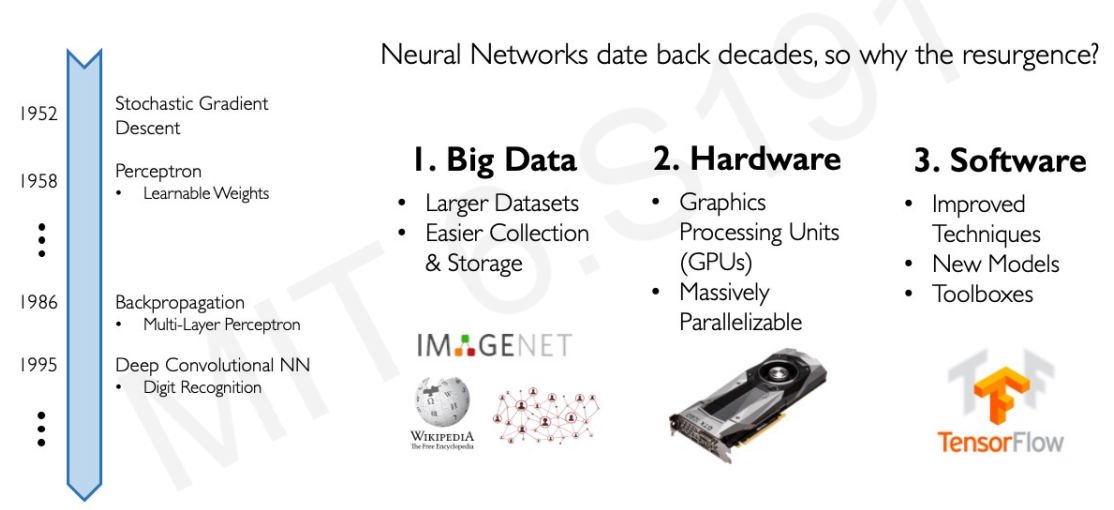
\includegraphics[width=1\textwidth,height=\textheight]{images/WhyDLNow.png}
Source: Alex Amini's `MIT Introduction to Deep Learning' course
(introtodeeplearning.com)

Success stories such as

\begin{itemize}
\item
  the development of self-driving cars,
\item
  the use of AI in medical diagnosis, and
\item
  the creation of personalized recommendations in online shopping
\end{itemize}

have also contributed to the widespread adoption of AI.

\hypertarget{comparison-with-traditional-machine-learning}{%
\subsubsection{Comparison with Traditional Machine
Learning}\label{comparison-with-traditional-machine-learning}}

A reasonable question is ``\emph{how are ArtificiaI Intelligence,
Machine Learning and Deep learning related}''?

A standard answer can be found in the image below that has a myriad
variations:

\begin{Shaded}
\begin{Highlighting}[]
\NormalTok{knitr}\SpecialCharTok{::}\FunctionTok{include\_graphics}\NormalTok{(}\StringTok{"images/AI{-}ML{-}DL{-}1.jpg"}\NormalTok{)}
\end{Highlighting}
\end{Shaded}

\begin{figure}[H]

{\centering 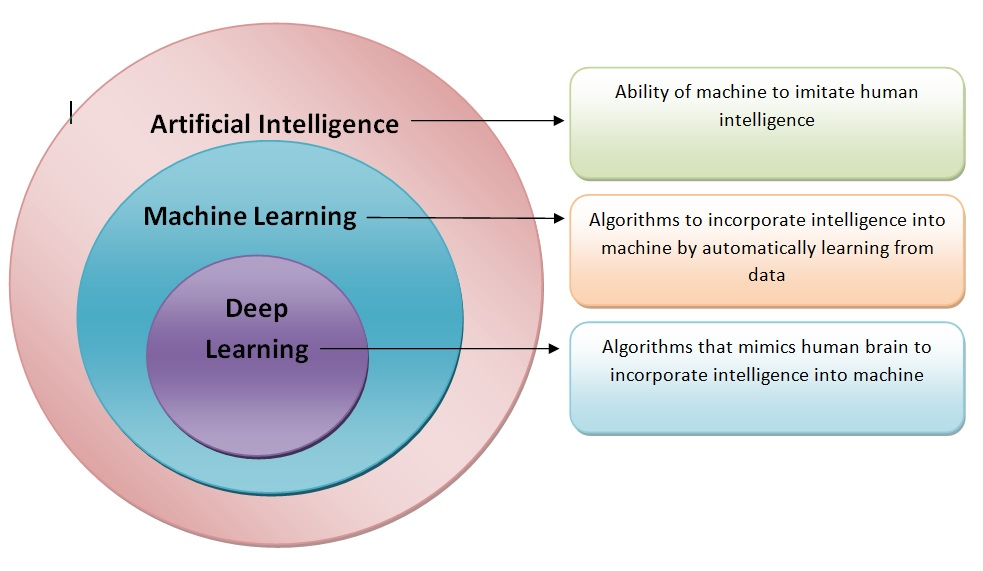
\includegraphics[width=1\textwidth,height=\textheight]{images/AI-ML-DL-1.jpg}

}

\end{figure}

We can keep three definitions:

\begin{itemize}
\item
  Artificial intelligence is the ability of a computer to perform tasks
  commonly associated with intelligent beings.
\item
  Machine learning is the study of algorithms that learn from examples
  and experience instead of relying on hard-coded rules and make
  predictions on new data
\item
  Deep learning is a subfield of machine learning focusing on learning
  data representations as successive successive layers of increasingly
  meaningful representations.
\end{itemize}

\begin{Shaded}
\begin{Highlighting}[]
\NormalTok{knitr}\SpecialCharTok{::}\FunctionTok{include\_graphics}\NormalTok{(}\StringTok{"images/ML\_vs\_DL{-}2.png"}\NormalTok{)}
\end{Highlighting}
\end{Shaded}

\begin{figure}[H]

{\centering 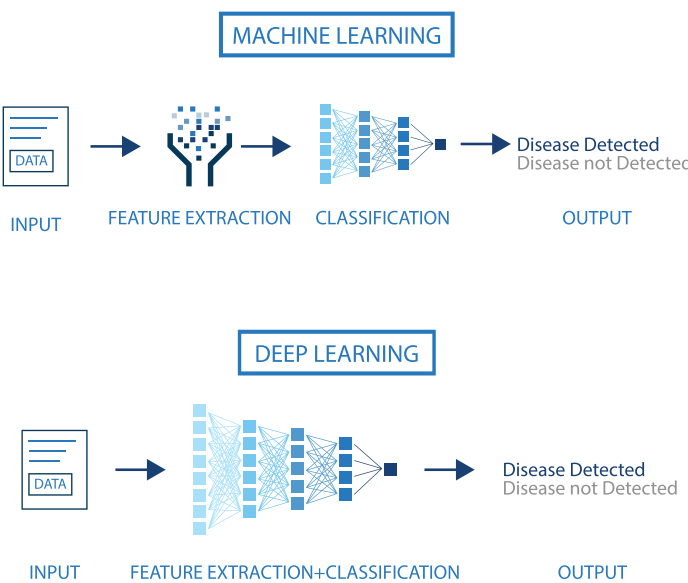
\includegraphics[width=1\textwidth,height=\textheight]{images/ML_vs_DL-2.png}

}

\end{figure}

We will be coming back to the difference between ML and DL, but two
strengths of DL that differentiate it from ML should be clear from the
beginning:

\begin{itemize}
\tightlist
\item
  DNN combine feature extraction and classification in a way that does
  not require (or dramatically decreases) human intervention.
\item
  The power of DNN requires in its ability to improve with data
  availability, without seemingly reaching plateaus as ML.
\end{itemize}

\begin{figure}

{\centering 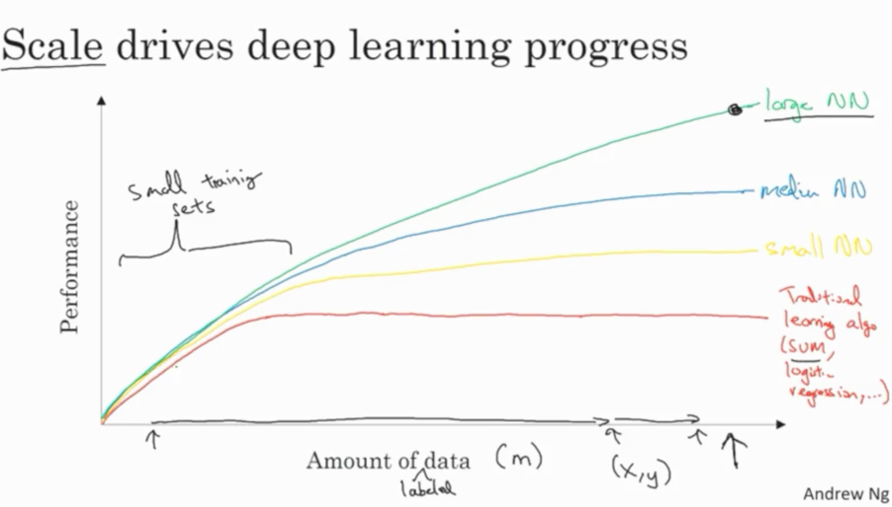
\includegraphics{images/PerformanceVsAmountOfData.png}

}

\caption{An illustration of the performance comparison between deep
learning (DL) and other machine learning (ML) algorithms, where DL
modeling from large amounts of data can increase the performance}

\end{figure}

\textbf{Deep learning is having a strong impact}

\begin{itemize}
\item
  Near-human-level image classification
\item
  Near-human-level speech transcription
\item
  Near-human-level handwriting transcription
\item
  Dramatically improved machine translation
\item
  Dramatically improved text-to-speech conversion
\item
  Digital assistants such as Google Assistant and Amazon Alexa
\item
  Near-human-level autonomous driving
\item
  Improved ad targeting, as used by Google, Baidu, or Bing
\item
  Improved search results on the web
\item
  Ability to answer natural language questions
\item
  Superhuman Go playing
\end{itemize}

According to {[}@chollet2022{]} \ldots{} ``\emph{we shouldn't believe
the short-term hype, but should believe in the long-term vision. It may
take a while for AI to be deployed to its true potential---a potential
the full extent of which no one has yet dared to dream---but AI is
coming, and it will transform our world in a fantastic way}''.

Once the introduction is ready we con move onto the building blocks of
neural networks, perceptrons.

\hypertarget{artificial-neural-networks}{%
\subsection{Artificial Neural
Networks}\label{artificial-neural-networks}}

\hypertarget{the-perceptron-the-building-block}{%
\subsubsection{The perceptron, the building
block}\label{the-perceptron-the-building-block}}

The perceptron, was introduced by Rosenblatt (one version of the
perceptron at least), as a mathematical model that might emulate a
neuron.

The idea is: \emph{how can we produce a model that given some inputs,
and an appropriate set of examples, learn to produce the desired
output}?

The first computational model of a neuron was proposed by Warren
MuCulloch (neuroscientist) and Walter Pitts (logician) in 1943.

\begin{figure}

{\centering 

\href{https://towardsdatascience.com/mcculloch-pitts-model-5fdf65ac5dd1}{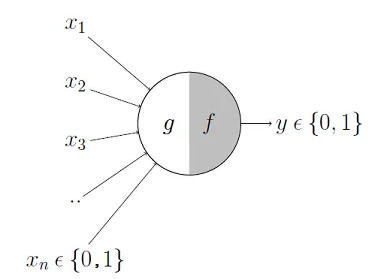
\includegraphics{images/MacCulloghPitts-Neuron.png}}

}

\end{figure}

It may be divided into 2 parts. The first part, \(g\),takes an input
(ahem dendrite ahem), performs an aggregation and based on the
aggregated value the second part, \(f\), makes a decision. See
\href{https://towardsdatascience.com/mcculloch-pitts-model-5fdf65ac5dd1}{the
source of this picture} for an illustration on how this can be used to
emulate logical operations such as AND, OR or NOT, but not XOR.

This first attempt to emulate neurons succeeded but with limitations:

\begin{itemize}
\item
  What about non-boolean (say, real) inputs?
\item
  What if all inputs are not equal?
\item
  What if we want to assign more importance to some inputs?
\item
  What about functions which are not linearly separable? Say XOR
  function
\end{itemize}

To overcome these limitations Frank Rosenblatt, an American
psychologist, proposed the classical perception model, the
\emph{artificial neuron}, in 1958. It is more generalized computational
model than the McCulloch-Pitts neuron where weights and thresholds can
be learnt over time.

The perceptron proposed by Rosenblatt this is very similar to an M-P
neuron but we take a weighted sum of the inputs and set the output as
one only when the sum is more than an arbitrary threshold
(\textbf{\emph{theta}}).

\begin{figure}

{\centering 

\href{https://towardsdatascience.com/perceptron-the-artificial-neuron-4d8c70d5cc8d}{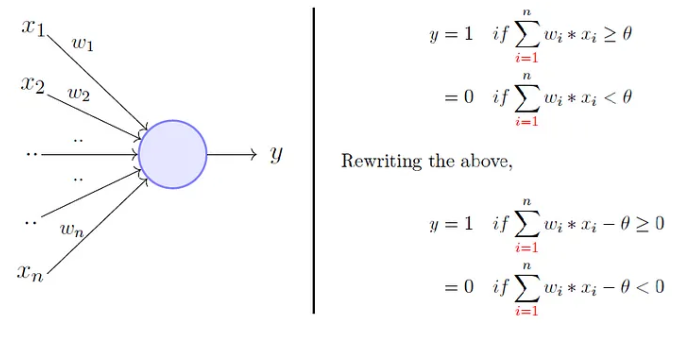
\includegraphics{images/RosenblattPerceptron1.png}}

}

\end{figure}

Additionally, instead of hand coding the thresholding parameter
\(\theta\), we add it as one of the inputs, with the weight
\(w_0=-\theta\) like shown below, which makes it learnable.

\begin{figure}

{\centering 

\href{https://towardsdatascience.com/perceptron-the-artificial-neuron-4d8c70d5cc8d}{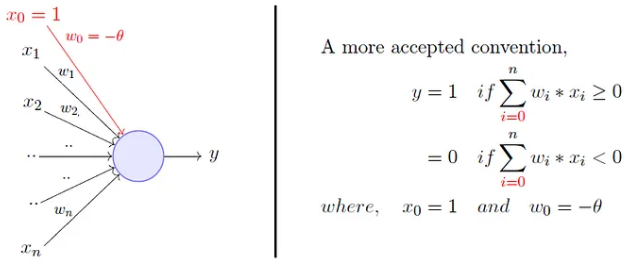
\includegraphics{images/RosenblattPerceptron2.png}}

}

\end{figure}

\begin{figure}

{\centering 

\href{https://towardsdatascience.com/perceptron-the-artificial-neuron-4d8c70d5cc8d}{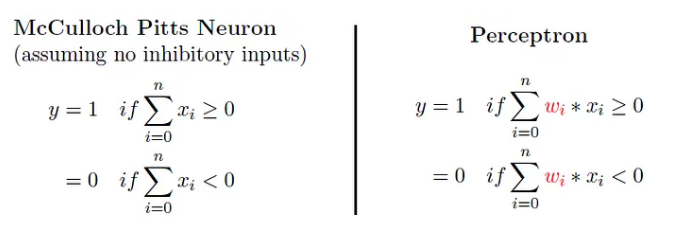
\includegraphics{images/McCullaughVSRosenblattPerceptron.png}}

}

\end{figure}

Now, while this is an improvement (because both the weights and the
threshold can be learned and the inputs can be real values) there is
still a drawback in that a single perceptron can only be used to
implement linearly separable functions.

Artificial Neural Networks improve on this by introducing
\emph{Activation Functions} which, eventually, can be non-linear.

\hypertarget{neurons-and-activation-functions}{%
\subsubsection{Neurons and Activation
Functions}\label{neurons-and-activation-functions}}

An activation function is a function that is added into an artificial
neurone in order to help it learn complex patterns in the data.

How come biological and artificial neurons come to compare?

Biological neurons are specialized cells in the central nervous system
that transmit electrical and chemical signals to communicate with each
other and the rest of the body.

On the other hand, artificial neurons are mathematical models used in
neural networks to process information.

In both biological and artificial neurons, the \textbf{activation
function} is what is responsible for \emph{deciding whether the neuron
activates or not based on the input it receives}.

\begin{itemize}
\tightlist
\item
  In the case of a biological neuron, the activation function is based
  on the release of neurotransmitters, which are chemical substances
  that transmit signals between nerve cells. When the electrical signal
  reaching the neuron exceeds a certain threshold, the neuron releases
  neurotransmitters, which are received by other neurons or cells in the
  body to continue the communication process.
\item
  On the other hand, in an artificial neuron, the activation function is
  a mathematical function applied to the neuron's input to produce an
  output. Like in the biological neuron, this activation function
  decides whether the neuron activates or not based on the input it
  receives.
\end{itemize}

\begin{Shaded}
\begin{Highlighting}[]
\NormalTok{knitr}\SpecialCharTok{::}\FunctionTok{include\_graphics}\NormalTok{(}\StringTok{"images/ActivationFunction0.png"}\NormalTok{)}
\end{Highlighting}
\end{Shaded}

\begin{figure}[H]

{\centering 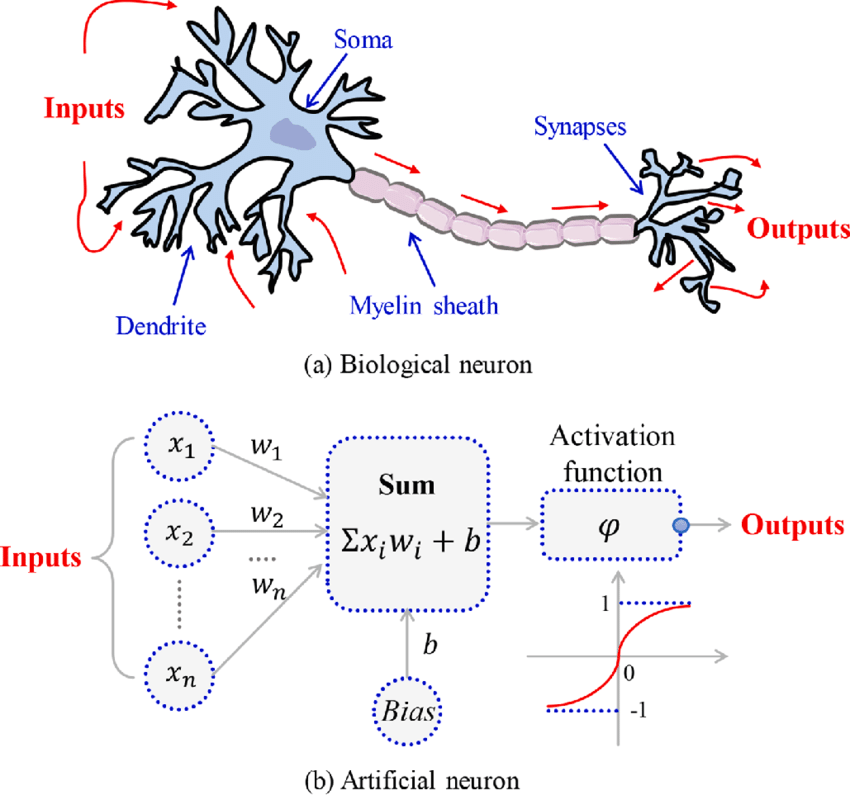
\includegraphics[width=1\textwidth,height=\textheight]{images/ActivationFunction0.png}

}

\end{figure}

\href{https://towardsdatascience.com/everything-you-need-to-know-about-activation-functions-in-deep-learning-models-84ba9f82c253}{Read
more here about activation functions.}

With all these inputs in mind we can now define an Artificial Neuron as
a \emph{computational unit} that - takes as input
\(x=(x_0,x_1,x_2,x_3)\) (\(x_0\) = +1, called bias), and - outputs
\(h_{\theta}(x) = f(\theta^\intercal x) = f(\sum_i \theta_ix_i)\), -
where \(f:\mathbb{R}\mapsto \mathbb{R}\) is called the
\textbf{activation function}.

The goal of the activation function is to provide the Neuron with
\emph{the capability of producing the required outputs}.

For instance, if the output has to be a probability, the activation
function will only produce values between 0 and 1.

With this idea in mind activation functions are chosen from a set of
pre-defined functions:

\begin{itemize}
\tightlist
\item
  the sigmoid function:
\end{itemize}

\[
f(z)=\frac{1}{1+e^{-z}}
\]

\begin{itemize}
\tightlist
\item
  the hyperbolic tangent, or \texttt{tanh}, function:
\end{itemize}

\[
f(z)=\frac{e^{z}-e^{-z}}{e^{z}+e^{-z}}
\]

The \texttt{tanh(z)} function is a rescaled version of the sigmoid, and
its output range is \([-1,1]\) instead of \([0,1]\).

Two useful properties to recall are that: - \emph{If} \(f(z)=1/(1+e^z)\)
is the sigmoid function, then its derivative is given by
\(f'(z)=f(z)(1-f(z))\).

\begin{itemize}
\item
  \emph{Similarly, if} \(f\) is the \texttt{tanh} function, then its
  derivative is given by \(f'(z)=1-(f(z))^2\).
\item
  In modern neural networks, the default recommendation is to use the
  \emph{rectified linear unit} or ReLU defined by the activation
  function \(f(z)=\max\{0,z\}\).
\end{itemize}

This function remains very close to a linear one, in the sense that is a
piecewise linear function with two linear pieces.

Because rectified linear units are nearly linear, they preserve many of
the properties that make linear models easy to optimize with gradient
based methods.

They also preserve many of the properties that make linear models
generalize well.

\href{https://medium.com/@shrutijadon/survey-on-activation-functions-for-deep-learning-9689331ba092}{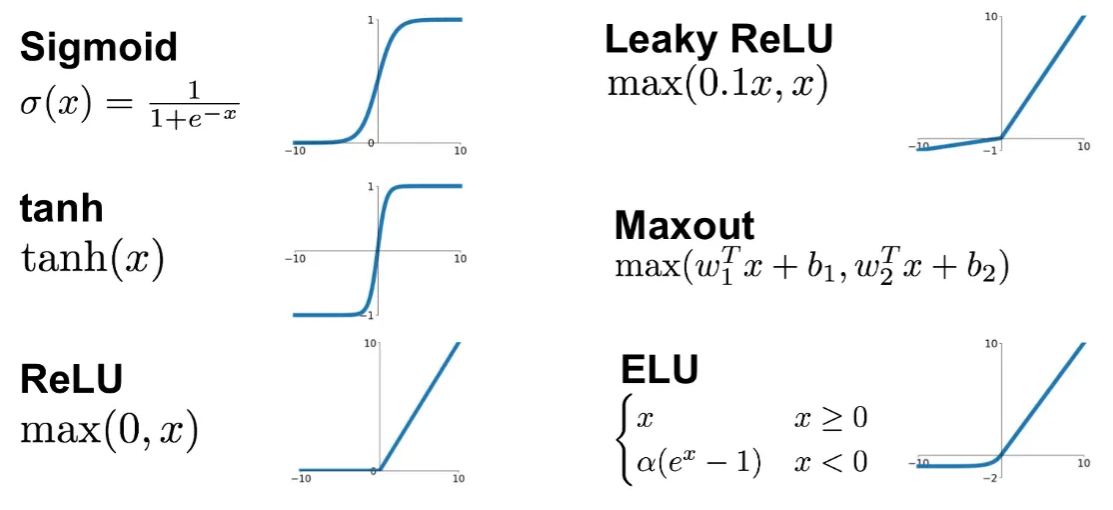
\includegraphics{images/ActivationFunctions.png}}.

\textbf{Putting alltogether} we have the following schematic
representation of an artificial neuron where
\(\Sigma=\left\langle w_{j}, x\right\rangle+ b_{j}\) and
\(\left\langle w_{j}, x\right\rangle\) represents the dot product
between vectors \(w\) and \(x\).

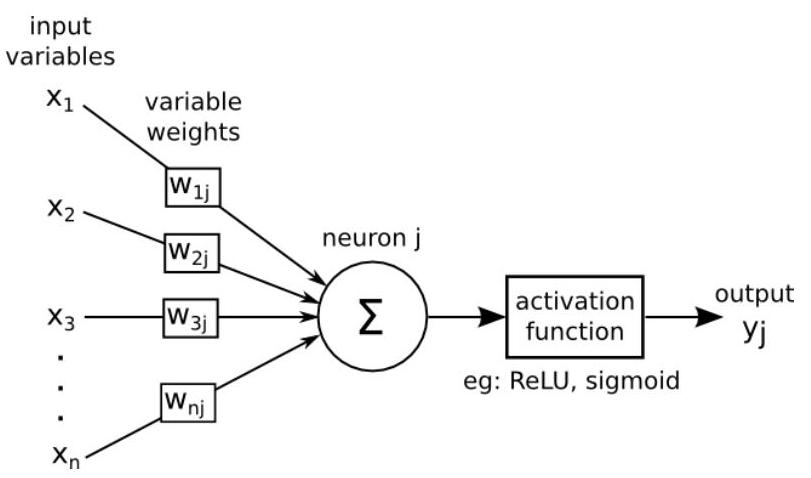
\includegraphics{images/ArtificialNeuron.png}

\hypertarget{multilayer-perceptrons}{%
\subsubsection{Multilayer perceptrons}\label{multilayer-perceptrons}}

A multilayer perceptron (or Artificial neural network) is a structure
composed by \emph{several hidden layers of neurons} where the output of
a neuron of a layer becomes the input of a neuron of the next layer.

Moreover, the output of a neuron can also be the input of a neuron of
the same layer or of neuron of previous layers (this is the case for
recurrent neural networks). On last layer, called output layer, we may
apply a different activation function as for the hidden layers depending
on the type of problems we have at hand : regression or classification.

The Figure below represents a neural network with three input variables,
one output variable, and two hidden layers.

\begin{Shaded}
\begin{Highlighting}[]
\NormalTok{knitr}\SpecialCharTok{::}\FunctionTok{include\_graphics}\NormalTok{(}\StringTok{"images/MultiLayer1.png"}\NormalTok{)}
\end{Highlighting}
\end{Shaded}

\begin{figure}[H]

{\centering 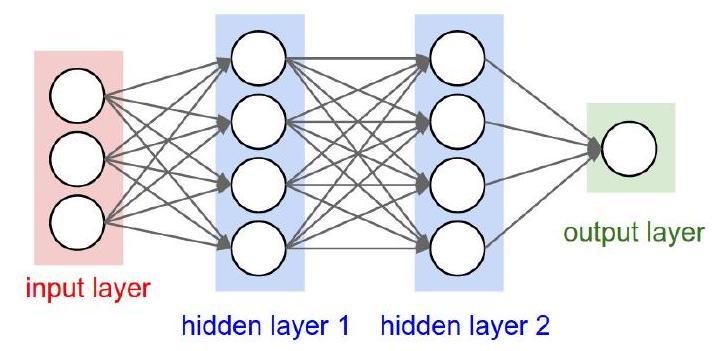
\includegraphics[width=1\textwidth,height=\textheight]{images/MultiLayer1.png}

}

\end{figure}

Multilayers perceptrons have a basic architecture since each unit (or
neuron) of a layer is linked to all the units of the next layer but has
no link with the neurons of the same layer.

The parameters of the architecture are:

\begin{itemize}
\tightlist
\item
  the number of hidden layers and
\item
  the number of neurons in each layer.
\end{itemize}

The activation functions are also to choose by the user. For the output
layer, as mentioned previously, the activation function is generally
different from the one used on the hidden layers. For example:.

\begin{itemize}
\tightlist
\item
  For regression, we apply no activation function on the output layer.
\item
  For binary classification, the output gives a prediction of
  \(\mathbb{P}(Y=1 / X)\) since this value is in \([0,1]\) and the
  sigmoid activation function is generally considered.
\item
  For multi-class classification, the output layer contains one neuron
  per class (i), giving a prediction of \(\mathbb{P}(Y=i / X)\). The sum
  of all these values has to be equal to 1. The sum of all these values
  has to be equal to 1.

  \begin{itemize}
  \tightlist
  \item
    A common choice for multi-class ANN is the \emph{softmax} activation
    function: \[
    \operatorname{softmax}(z)_{i}=\frac{\exp \left(z_{i}\right)}{\sum_{j} \exp \left(z_{j}\right)}
    \]
  \end{itemize}
\end{itemize}

\hypertarget{an-example}{%
\subsection{An example}\label{an-example}}

In this example we train and use a ``shallow neural network'', called
this way in contrast with ``deep neural networks''.

We will use the \texttt{neuralnet} R package, which is not intended to
work with deep neural networks, to build a simple neural network to
predict if a type of stock pays dividends or not.

\begin{Shaded}
\begin{Highlighting}[]
\ControlFlowTok{if}\NormalTok{ (}\SpecialCharTok{!}\FunctionTok{require}\NormalTok{(neuralnet)) }
  \FunctionTok{install.packages}\NormalTok{(}\StringTok{"neuralnet"}\NormalTok{, }\AttributeTok{dep=}\ConstantTok{TRUE}\NormalTok{)}
\ControlFlowTok{if}\NormalTok{ (}\SpecialCharTok{!}\FunctionTok{require}\NormalTok{(caret)) }
  \FunctionTok{install.packages}\NormalTok{(}\StringTok{"caret"}\NormalTok{, }\AttributeTok{dep=}\ConstantTok{TRUE}\NormalTok{)}
\end{Highlighting}
\end{Shaded}

The data for the example are the \texttt{dividendinfo.csv} dataset,
available from: \url{https://github.com/MGCodesandStats/datasets}

\begin{Shaded}
\begin{Highlighting}[]
\NormalTok{mydata }\OtherTok{\textless{}{-}} \FunctionTok{read.csv}\NormalTok{(}\StringTok{"https://raw.githubusercontent.com/MGCodesandStats/datasets/master/dividendinfo.csv"}\NormalTok{)}
\FunctionTok{str}\NormalTok{(mydata)}
\end{Highlighting}
\end{Shaded}

\begin{verbatim}
'data.frame':   200 obs. of  6 variables:
 $ dividend       : int  0 1 1 0 1 1 1 0 1 1 ...
 $ fcfps          : num  2.75 4.96 2.78 0.43 2.94 3.9 1.09 2.32 2.5 4.46 ...
 $ earnings_growth: num  -19.25 0.83 1.09 12.97 2.44 ...
 $ de             : num  1.11 1.09 0.19 1.7 1.83 0.46 2.32 3.34 3.15 3.33 ...
 $ mcap           : int  545 630 562 388 684 621 656 351 658 330 ...
 $ current_ratio  : num  0.924 1.469 1.976 1.942 2.487 ...
\end{verbatim}

\hypertarget{data-preprocessing}{%
\subsubsection{Data preprocessing}\label{data-preprocessing}}

One of the most important procedures when forming a neural network is
data normalization. This involves adjusting the data to a common scale
so as to accurately compare predicted and actual values. Failure to
normalize the data will typically result in the prediction value
remaining the same across all observations, regardless of the input
values.

We can do this in two ways in R:

\begin{itemize}
\tightlist
\item
  Scale the data frame automatically using the scale function in R
\item
  Transform the data using a max-min normalization technique
\end{itemize}

In this example We implement the max-min normalization technique.

See
\href{https://vitalflux.com/data-science-scale-normalize-numeric-data-using-r/}{this
link} for further details on how to use the normalization function.

\begin{Shaded}
\begin{Highlighting}[]
\NormalTok{normalize }\OtherTok{\textless{}{-}} \ControlFlowTok{function}\NormalTok{(x) \{}
  \FunctionTok{return}\NormalTok{ ((x }\SpecialCharTok{{-}} \FunctionTok{min}\NormalTok{(x)) }\SpecialCharTok{/}\NormalTok{ (}\FunctionTok{max}\NormalTok{(x) }\SpecialCharTok{{-}} \FunctionTok{min}\NormalTok{(x)))}
\NormalTok{\}}
\NormalTok{normData }\OtherTok{\textless{}{-}} \FunctionTok{as.data.frame}\NormalTok{(}\FunctionTok{lapply}\NormalTok{(mydata, normalize))}
\end{Highlighting}
\end{Shaded}

As usually, the dataset is separated in a training and a test set. The
training set contains a random selection with and (arbitrary) 66\% of
the observations.

\begin{Shaded}
\begin{Highlighting}[]
\NormalTok{perc2Train }\OtherTok{\textless{}{-}} \DecValTok{2}\SpecialCharTok{/}\DecValTok{3}
\NormalTok{ssize }\OtherTok{\textless{}{-}} \FunctionTok{nrow}\NormalTok{(normData)}
\FunctionTok{set.seed}\NormalTok{(}\DecValTok{12345}\NormalTok{)}
\NormalTok{data\_rows }\OtherTok{\textless{}{-}} \FunctionTok{floor}\NormalTok{(perc2Train }\SpecialCharTok{*}\NormalTok{ssize)}
\NormalTok{train\_indices }\OtherTok{\textless{}{-}} \FunctionTok{sample}\NormalTok{(}\FunctionTok{c}\NormalTok{(}\DecValTok{1}\SpecialCharTok{:}\NormalTok{ssize), data\_rows)}
\NormalTok{trainset }\OtherTok{\textless{}{-}}\NormalTok{ normData[train\_indices,]}
\NormalTok{testset }\OtherTok{\textless{}{-}}\NormalTok{ normData[}\SpecialCharTok{{-}}\NormalTok{train\_indices,]}
\end{Highlighting}
\end{Shaded}

The \texttt{trainset} set will be used to train the network and the
\texttt{testset} set one will be used to evaluate it.

\hypertarget{training-a-neural-network}{%
\subsubsection{Training a neural
network}\label{training-a-neural-network}}

Setting the parameters of a neural network requires experience and
understanding of their meaning, and even so, canges in the parameters
can lead to similar results.

We create a simple NN with two hidden layers, with 3 and 2 neurons
respectively. This is specified in the \texttt{hidden} parameter. For
other parameters see
\href{https://www.rdocumentation.org/packages/neuralnet/versions/1.44.2/topics/neuralnet}{the
package help}.

\begin{Shaded}
\begin{Highlighting}[]
\CommentTok{\# Neural Network}
\FunctionTok{library}\NormalTok{(neuralnet)}
\NormalTok{nn }\OtherTok{\textless{}{-}} \FunctionTok{neuralnet}\NormalTok{(dividend }\SpecialCharTok{\textasciitilde{}}\NormalTok{ fcfps }\SpecialCharTok{+}\NormalTok{ earnings\_growth }\SpecialCharTok{+}\NormalTok{ de }\SpecialCharTok{+}\NormalTok{ mcap }\SpecialCharTok{+}\NormalTok{ current\_ratio, }
                \AttributeTok{data=}\NormalTok{trainset, }
                \AttributeTok{hidden=}\FunctionTok{c}\NormalTok{(}\DecValTok{3}\NormalTok{,}\DecValTok{2}\NormalTok{), }
                \AttributeTok{linear.output=}\ConstantTok{FALSE}\NormalTok{, }
                \AttributeTok{threshold=}\FloatTok{0.01}\NormalTok{)}
\end{Highlighting}
\end{Shaded}

The output of the procedure is a neural network with estimated weights.

This can be seen with a \texttt{plot} function (including the
\texttt{rep} argument).

\begin{Shaded}
\begin{Highlighting}[]
\FunctionTok{plot}\NormalTok{(nn, }\AttributeTok{rep =} \StringTok{"best"}\NormalTok{)}
\end{Highlighting}
\end{Shaded}

\begin{figure}[H]

{\centering 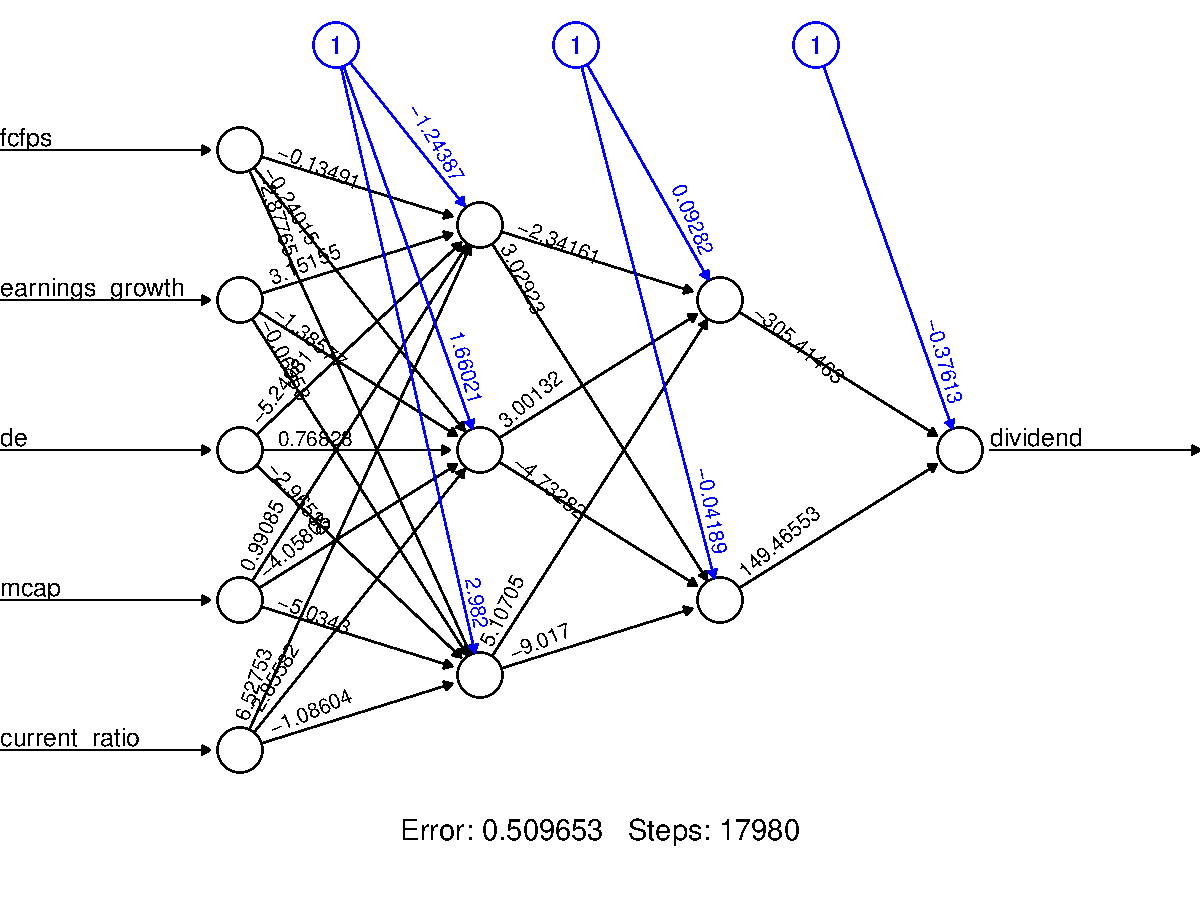
\includegraphics{Introduction_to_Deep_Learning_files/figure-pdf/unnamed-chunk-11-1.pdf}

}

\end{figure}

The object \texttt{nn}contains information the weights and the results
although it is not particularly clear or useful.

\begin{Shaded}
\begin{Highlighting}[]
\FunctionTok{summary}\NormalTok{(nn)}
\end{Highlighting}
\end{Shaded}

\begin{verbatim}
                    Length Class      Mode    
call                  6    -none-     call    
response            133    -none-     numeric 
covariate           665    -none-     numeric 
model.list            2    -none-     list    
err.fct               1    -none-     function
act.fct               1    -none-     function
linear.output         1    -none-     logical 
data                  6    data.frame list    
exclude               0    -none-     NULL    
net.result            1    -none-     list    
weights               1    -none-     list    
generalized.weights   1    -none-     list    
startweights          1    -none-     list    
result.matrix        32    -none-     numeric 
\end{verbatim}

\begin{Shaded}
\begin{Highlighting}[]
\NormalTok{nn}\SpecialCharTok{$}\NormalTok{result.matrix}
\end{Highlighting}
\end{Shaded}

\begin{verbatim}
                                     [,1]
error                        5.096531e-01
reached.threshold            9.874263e-03
steps                        1.798000e+04
Intercept.to.1layhid1       -1.243872e+00
fcfps.to.1layhid1           -1.349137e-01
earnings_growth.to.1layhid1  3.151554e+00
de.to.1layhid1              -5.249806e+00
mcap.to.1layhid1             9.908495e-01
current_ratio.to.1layhid1    6.527535e+00
Intercept.to.1layhid2        1.660208e+00
fcfps.to.1layhid2           -2.401517e-01
earnings_growth.to.1layhid2 -1.385771e+00
de.to.1layhid2               7.682849e-01
mcap.to.1layhid2            -4.058053e+00
current_ratio.to.1layhid2   -2.855816e+00
Intercept.to.1layhid3        2.982002e+00
fcfps.to.1layhid3           -2.877651e+00
earnings_growth.to.1layhid3 -6.957763e-02
de.to.1layhid3              -2.965334e+00
mcap.to.1layhid3            -5.034300e+00
current_ratio.to.1layhid3   -1.086037e+00
Intercept.to.2layhid1        9.282087e-02
1layhid1.to.2layhid1        -2.341614e+00
1layhid2.to.2layhid1         3.001315e+00
1layhid3.to.2layhid1         5.107051e+00
Intercept.to.2layhid2       -4.188729e-02
1layhid1.to.2layhid2         3.029232e+00
1layhid2.to.2layhid2        -4.732821e+00
1layhid3.to.2layhid2        -9.017001e+00
Intercept.to.dividend       -3.761263e-01
2layhid1.to.dividend        -3.054146e+02
2layhid2.to.dividend         1.494655e+02
\end{verbatim}

\hypertarget{model-evaluation}{%
\subsubsection{Model evaluation}\label{model-evaluation}}

A prediction for each value in the \texttt{testset} dataset can be built
with the \texttt{compute} function.

\begin{Shaded}
\begin{Highlighting}[]
\CommentTok{\#Test the resulting output}
\NormalTok{temp\_test }\OtherTok{\textless{}{-}} \FunctionTok{subset}\NormalTok{(testset, }\AttributeTok{select =}
                      \FunctionTok{c}\NormalTok{(}\StringTok{"fcfps"}\NormalTok{,}\StringTok{"earnings\_growth"}\NormalTok{, }
                        \StringTok{"de"}\NormalTok{, }\StringTok{"mcap"}\NormalTok{, }\StringTok{"current\_ratio"}\NormalTok{))}
\FunctionTok{head}\NormalTok{(temp\_test)}
\end{Highlighting}
\end{Shaded}

\begin{verbatim}
       fcfps earnings_growth        de       mcap current_ratio
9  0.4929006      0.52417860 0.7862595 0.79741379   0.662994637
19 0.8722110      0.89705139 0.5190840 0.31465517   0.631284474
22 0.0811359      0.68272957 0.4554707 0.05747126   0.000785556
26 0.4077079      0.07649537 0.6310433 0.70977011   0.379642293
27 0.4279919      0.70362258 0.1882952 0.30603448   0.628283435
29 0.3509128      0.74203875 0.6030534 0.53017241   0.543404499
\end{verbatim}

\begin{Shaded}
\begin{Highlighting}[]
\NormalTok{nn.results }\OtherTok{\textless{}{-}} \FunctionTok{compute}\NormalTok{(nn, temp\_test)}
\NormalTok{results }\OtherTok{\textless{}{-}} \FunctionTok{data.frame}\NormalTok{(}\AttributeTok{actual =} 
\NormalTok{                  testset}\SpecialCharTok{$}\NormalTok{dividend, }
                  \AttributeTok{prediction =}\NormalTok{ nn.results}\SpecialCharTok{$}\NormalTok{net.result)}
\FunctionTok{head}\NormalTok{(results)}
\end{Highlighting}
\end{Shaded}

\begin{verbatim}
   actual    prediction
9       1  1.000000e+00
19      1  1.000000e+00
22      0 5.442517e-133
26      0  6.801894e-35
27      1  4.548179e-10
29      1  1.000000e+00
\end{verbatim}

A confusion matrix can be built to evaluate the predictive ability of
the network:

\begin{Shaded}
\begin{Highlighting}[]
\NormalTok{roundedresults}\OtherTok{\textless{}{-}}\FunctionTok{sapply}\NormalTok{(results,round,}\AttributeTok{digits=}\DecValTok{0}\NormalTok{)}
\NormalTok{roundedresultsdf}\OtherTok{=}\FunctionTok{data.frame}\NormalTok{(roundedresults)}
\FunctionTok{attach}\NormalTok{(roundedresultsdf)}
\NormalTok{confMat}\OtherTok{\textless{}{-}}\NormalTok{ caret}\SpecialCharTok{::}\FunctionTok{confusionMatrix}\NormalTok{(}\FunctionTok{table}\NormalTok{(actual, prediction))}
\NormalTok{confMat}
\end{Highlighting}
\end{Shaded}

\begin{verbatim}
Confusion Matrix and Statistics

      prediction
actual  0  1
     0 34  2
     1  6 25
                                         
               Accuracy : 0.8806         
                 95% CI : (0.7782, 0.947)
    No Information Rate : 0.597          
    P-Value [Acc > NIR] : 3.405e-07      
                                         
                  Kappa : 0.7577         
                                         
 Mcnemar's Test P-Value : 0.2888         
                                         
            Sensitivity : 0.8500         
            Specificity : 0.9259         
         Pos Pred Value : 0.9444         
         Neg Pred Value : 0.8065         
             Prevalence : 0.5970         
         Detection Rate : 0.5075         
   Detection Prevalence : 0.5373         
      Balanced Accuracy : 0.8880         
                                         
       'Positive' Class : 0              
                                         
\end{verbatim}

\hypertarget{some-mathematics-behind-ann}{%
\section{Some mathematics behind
ANN}\label{some-mathematics-behind-ann}}

\hypertarget{mathematical-formulation}{%
\subsection{Mathematical formulation}\label{mathematical-formulation}}

\begin{itemize}
\item
  An ANN is a predictive model whose functioning and properties can be
  mathematically characterized.
\item
  In practice this means describing

  \begin{itemize}
  \tightlist
  \item
    The ANN as a (non linear) function.
  \item
    The (optimization) process for estimating the weights.
  \end{itemize}
\item
  Estimation is done by minimizing an appropriate loss function which
  requires

  \begin{itemize}
  \tightlist
  \item
    An appropriate procedure: \emph{gradient based optimization}
  \item
    A method for computing the required derivatives:
    \emph{back-propagation}.
  \end{itemize}
\end{itemize}

\hypertarget{mathematical-formulation-of-the-ann}{%
\subsection{Mathematical formulation of the
ANN}\label{mathematical-formulation-of-the-ann}}

We will use a concrete model to explain the concepts, which can be
easily generalized to more neurons and layers.

Consider the following simple ANN:

Consider the following ANN:

\begin{Shaded}
\begin{Highlighting}[]
\NormalTok{knitr}\SpecialCharTok{::}\FunctionTok{include\_graphics}\NormalTok{(}\StringTok{"images/nn.jpg"}\NormalTok{)}
\end{Highlighting}
\end{Shaded}

\begin{figure}[H]

{\centering 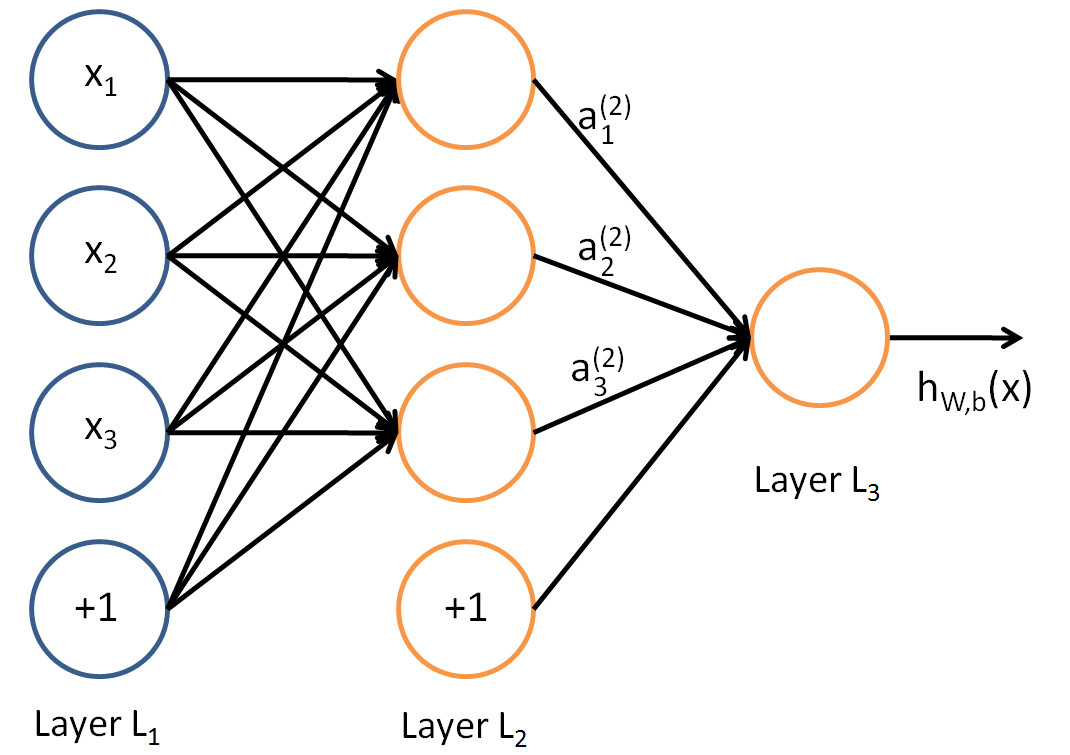
\includegraphics[width=1\textwidth,height=\textheight]{images/nn.jpg}

}

\end{figure}

\begin{itemize}
\tightlist
\item
  The circles labeled +1 are called bias units, and correspond to the
  intercept, here named \emph{bias} term.
\item
  The leftmost layer of the network is called the \emph{input layer}.
\item
  The rightmost layer is the \emph{output} layer (which, in this
  example, has only one node).
\item
  The middle layer(s) is(are) called the \emph{hidden layer(s)}, because
  its values are not observed in the training set.
\end{itemize}

So our example network has:

\begin{itemize}
\tightlist
\item
  The input layer with 3 input units (not counting the bias unit),
\item
  1 hidden layer with 3 hidden units, and
\item
  The output layer with 1 output unit.
\end{itemize}

\hypertarget{a-logistic-regression-ann}{%
\subsubsection{A logistic regression
ANN}\label{a-logistic-regression-ann}}

This ANN can be use to build a logistic regression model:

\begin{itemize}
\item
  From input layer to layer 2: non-linear transformation
  --\textgreater{} new set of complex features.
\item
  From layer 2 to output layer use a sigmoid activation function to
  produce the following output from the set of \emph{complex features}.
\end{itemize}

\[
\mbox{The output is: }h_{\theta}(x)=\frac{1}{1+e^{-\theta^\intercal x}}
\]

Recall that, the logistic regression model is:

\[
\log\frac{p(Y=1|x)}{1-p(Y=1|x)}=\theta^\intercal x
\]

Isolating \(p(Y=1|x)\) and taking logs in both sides, we have:

\[
\frac{p(Y=1|x)}{1-p(Y=1|x)}=e^{\theta^\intercal x}
\]

Thus \[
p(Y=1|x)=\frac{e^{\theta^\intercal x}}{1+e^{\theta^\intercal x}}=\frac{1}{1+e^{-\theta^\intercal x}}
\]

That is, \emph{when the activation function of the output node is the
sigmoid activation function, the output coincides with a logistic
regression on complex features}

\begin{itemize}
\tightlist
\item
  And, with \(h_{\theta}(x)\), the output of the NN, we are estimating
  \(p(Y=1|x)\).
\end{itemize}

\hypertarget{parametrizing-an-ann}{%
\subsection{Parametrizing an ANN}\label{parametrizing-an-ann}}

\begin{itemize}
\item
  Let \(n_l\) denote the number of layers in our network, thus \(n_l=3\)
  in our example.
\item
  Label layer \(l\) as \(L_l\), so layer \(L_1\) is the input layer, and
  layer \(L_{n_l}=L_3\) the output layer.
\item
  Our neural network has parameters:
  \(\Theta=(\Theta^{(1)},\Theta^{(2)})\), where we will write
  \(\theta^{(l)}_{ij}\) to denote the parameter (or weight) associated
  with the connection between unit \(j\) in layer \(l\), and unit \(i\)
  in layer \(l+1\).
\item
  Thus, in our example, we have:

  \begin{itemize}
  \tightlist
  \item
    \(\Theta^{(1)}\in\mathbb{R}^{3\times 4}\), and
  \item
    \(\Theta^{(2)}\in\mathbb{R}^{1\times 4}\).
  \end{itemize}
\end{itemize}

Note that bias units don't have inputs or connections going into them,
since they always output the value +1.

We also let \(s_l\) denote the number of nodes in layer \(l\) (not
counting the bias unit).

Now, write \(a^{(l)}_i\) to denote the activation (meaning output value)
of unit \(i\) in layer \(l\).

For \(l=1\), we also use \(a^{(1)}_i=x_i\) to denote the \(i\)-th input.

Given a fixed setting of the parameters \(\Theta\), our neural network
defines a model \(h_{\Theta}(x)\) that outputs a real number.

We can now see \emph{how these weights are used to produce the output}:

given by: \begin{eqnarray}
a_1^{(2)}&=&f(\theta_{10}^{(1)}+\theta_{11}^{(1)}x_1+\theta_{12}^{(1)}x_2+\theta_{13}^{(1)}x_3)\\
a_2^{(2)}&=&f(\theta_{20}^{(1)}+\theta_{21}^{(1)}x_1+\theta_{22}^{(1)}x_2+\theta_{23}^{(1)}x_3)\\
a_3^{(2)}&=&f(\theta_{30}^{(1)}+\theta_{31}^{(1)}x_1+\theta_{32}^{(1)}x_2+\theta_{33}^{(1)}x_3)\\
h_{\Theta}(x)&=&a_1^{(3)}=f(\theta_{10}^{(2)}+\theta_{11}^{(2)}a_1^{(2)}+\theta_{12}^{(2)}a_2^{(2)}+\theta_{13}^{(2)}a_3^{(2)})
\end{eqnarray}

Now, letting \(z_i^{(l)}\) denote the total weighted sum of inputs to
unit \(i\) in layer \(l\), including the bias term \[
z_i^{(2)}=\theta_{i0}^{(1)}+\theta_{i1}^{(1)}x_1+\theta_{i2}^{(1)}x_2+\theta_{i3}^{(1)}x_3,
\] the output becomes: \(a_i^{(l)}=f(z_i^{(l)})\).

\hypertarget{compacting-notation}{%
\subsection{Compacting notation}\label{compacting-notation}}

\begin{itemize}
\item
  Note that this easily lends itself to a more compact notation.
\item
  Extending the activation function \(f(\cdot)\) to apply to vectors in
  an elementwise fashion: \[
  f([z_1,z_2,z_3]) = [f(z_1), f(z_2),f(z_3)],
  \]
\end{itemize}

then we can write the previous equations more compactly as:

\begin{eqnarray}
z^{(2)}&=&\Theta^{(1)}x\nonumber\\
a^{(2)}&=&f(z^{(2)})\nonumber\\
z^{(3)}&=&\Theta^{(2)}a^{(2)}\nonumber\\
h_{\Theta}(x)&=&a^{(3)}=f(z^{(3)})\nonumber
\end{eqnarray}

\begin{itemize}
\item
  More generally, recalling that we also use \(a^{(1)}=x\) to also
  denote the values from the input layer,
\item
  then given layer \(l\)'s activations \(a^{(l)}\), we can compute layer
  \(l+1\)'s activations \(a^{(l+1)}\) as:
\end{itemize}

\begin{eqnarray}
z^{(l+1)}&=&\Theta^{(l)}a^{(l)}\\
a^{(l+1)}&=&f(z^{(l+1)})
\end{eqnarray}

This can be used to provide a matrix representation for the weighted sum
of inputs of all neurons:

\[
z^{(l+1)}=
\begin{bmatrix}
z_1^{(l+1)}\\
z_2^{(l+1)}\\
\vdots\\
z_{s_{l+1}}^{(l)}
\end{bmatrix}=
\begin{bmatrix}
\theta_{10}^{(l)}& \theta_{11}^{(l)}&\theta_{12}^{(l)}&...&\theta_{1s_{l}}^{(l)}&\\
\theta_{20}^{(l)}& \theta_{21}^{(l)}&\theta_{22}^{(l)}&...&\theta_{2s_{l}}^{(l)}&\\
\vdots & \vdots& \vdots & \vdots & \vdots\\
\theta_{s_{l+1}0}^{(l)}& \theta_{s_{l+1}1}^{(l)}&\theta_{s_{l+1}2}^{(l)}&...&\theta_{s_{l+1}s_{l}}^{(l)}&\\
\end{bmatrix}
\cdot\begin{bmatrix}
1\\
a_1^{(l)}\\
a_2^{(l)}\\
\vdots\\
a_{s_l}^{(l)}
\end{bmatrix}
\]

So that, the activation is then:

\[
a^{(l+1)}=
\begin{bmatrix}
a_1^{(l+1)}\\
a_2^{(l+1)}\\
\vdots\\
a_{s_{l+1}}^{(l)}
\end{bmatrix}=f(z^{(l+1)})=\begin{bmatrix}
f(z_1^{(l+1)})\\
f(z_2^{(l+1)})\\
\vdots\\
f(z_{s_{l+1}}^{(l)})
\end{bmatrix}
\]

\hypertarget{references-and-resources}{%
\section{References and resources}\label{references-and-resources}}



\end{document}
